\documentclass{article}
\renewcommand{\familydefault}{\sfdefault}
\usepackage{helvet}
\usepackage[utf8]{inputenc}

\usepackage{graphicx}
\graphicspath{{images/}}

\usepackage{caption}
\usepackage{subcaption}
\PassOptionsToPackage{hyphens}{url}\usepackage{hyperref}
\def\UrlOrds{\do\*\do\-\do\~\do\'\do\"\do\-}%
\usepackage{float}
\usepackage{gensymb}
\usepackage{amsmath}
\graphicspath{{images/}}
\usepackage[margin=1.0in]{geometry}

\begin{document}
\begin{titlepage}

\newcommand{\HRule}{\rule{\linewidth}{0.5mm}} % Defines a new command for the horizontal lines, change thickness here

\center % Center everything on the page
\textsc{\LARGE University of Edinburgh}\\[1.5cm] % Name of your university/college
\textsc{\Large System Design Project}\\[0.5cm] % Major heading such as course name
\date{January 2017}
\textsc{\large }\\[0.5cm] % Minor heading such as course title
\HRule \\[0.4cm]
{ \huge \bfseries Progress Report}\\[0.4cm] % Title of your document
\HRule \\[1.5cm]
\begin{minipage}{0.7\textwidth}
\begin{flushleft} \large
\emph{Group 10 Members:}\\
s1368635 \textsc{Deirdre Bringas}
\\s1452672 \textsc{Demetra Charalambous}
\\s1411707 \textsc{Joshua Green}
\\s1342226 \textsc{Nicholas Georgiou}
\\s1431686 \textsc{Tom Lutzeyer}
\\s1421057 \textsc{Titas Skrebe}
\\s1441731 \textsc{Vlad Buzatu}
\end{flushleft}
\end{minipage}\\[4cm]
\\
\textsc{\Large NIGEL'S PHOTO}\\[0.5cm] 

\end{titlepage}

%-------------Introduction Section--------------------------------------------%
\newpage


\section{Introduction}
In the contents of the course "System Design Project" we were asked to build and implement the code of a robot by using Lego, an Arduino and our programming skills in order to play two-a-side football, loosely based on the Robocup competition. Firstly, we have been assigned to group number 10 (which consists of the members of our group whose names can be found in the cover page of this report). After the third friendly match we will have to cooperate with group number 9 as they will be our teammates in the league, forming "team E". Starting from the first week of the semester, we were allocated several individual, group and team tasks. These tasks would help us achieve our main goal, which is having a fully-functional robot that can play football according to the rules of the course. This report aims to cover how, as a group, we set out to tackle this project. It contains information on how we communicate, how tasks are allocated, when meetings are carried out, and how our progress is tracked. It also includes information about how we allocate and use resources, including our budget as well as a risk assessment of problems that we have or possibly will face.

\section{Organisation}
\subsection{Communication}
A variety of ideas were put forward in regards to our communication method. Among others Facebook messenger, email, an irc channel, and Slack were the most popular. As mutually agreed, Slack was selected as the most appropriate method of communication. It allows for uploading files and is the platform used for general communication amongst the SDP students and mentors. A Google calendar was also set up, where all the group, "team E", mentor meetings and milestones will be continuously added. This will allow all members of the group to keep track of dates and times of relevant events to attend. The project manager (for whom more details can be found in the next section) is in direct contact with our mentor, as well as our group members, keeping track of how the work is distributed, if everyone is meeting their deadlines and arranging the several meetings.

\subsection{Task Allocation}
Task allocations were carried out once we decided on our goals for this project. These goals included; having a working design for our robot by the first friendly, being able to catch the ball, turn towards goal and shoot, and having a working vision system.
With clear goals in mind, we set out to allocate each member of the group a task, both individual and group tasks. We decided that having a project manager would be essential for group coordination and organisation. The role was assigned to Deirdre. With a project manager in place further allocations were carried out.Titas and Joshua chose to work on the hardware portion of the project, with Demetra, Nicholas, Tom, Deirdre and Vlad working on the software part of the project. Once everyone was allocated to a section of the project, the next step was to decide what each person would work on and what deadlines would be set for delivering the product. This was done by looking at what had to be done for each milestone and producing a temporary table in which everyone was assigned a task and a date by which this would be completed. This table is a rough representation of how tasks will be completed as changes in the implementation of the robot might appear because of unforeseen issues. Nonetheless it is a useful and efficient way of making sure all members have a target to work towards. In Figure 1, a single group member's draft table is shown, roughly displaying the tasks until the second friendly match.

\begin{figure}[H]
	\centering
	\begin{minipage}{1\textwidth}
		\centering
		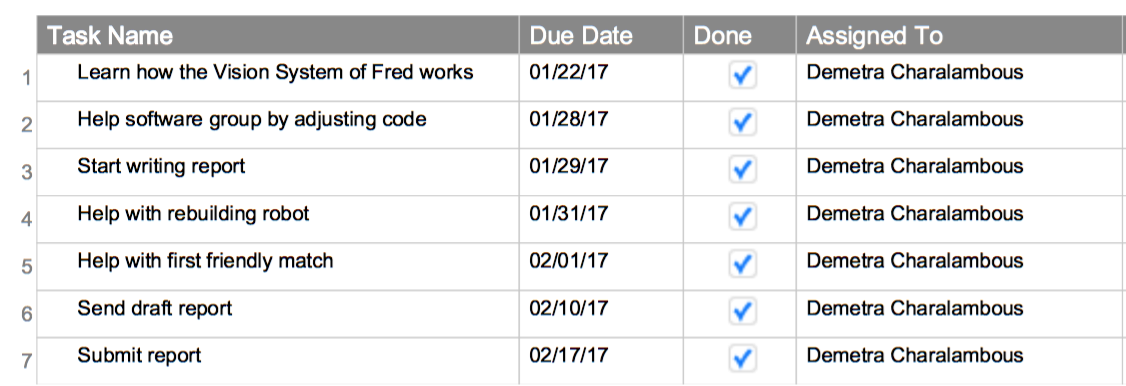
\includegraphics[width=16cm, height=6cm]{task_D.png}\\
		\caption{Example of individual temporary task table}
	\end{minipage}%
\end{figure}

We have also constructed a chart displaying how the members of the group are allocated in each sub-group. Sub-groups are smaller groups of group 10 which their members have tasks in common e.g. hardware group. After each friendly match we have a group meeting where we talk about what is required to do next and each member's tasks. During these meetings, responsibilities are assigned and the group is each time divided into sub-groups. In the first meeting we decided that an equal number of members in each sub-group would be ideal, as both hardware and software were of major importance. We also planned ahead and started the process report with two members of the group working on it (Figure 1 - part A). The first friendly match demonstrated that working on our overall strategy was key for the next match, thus more members were focusing on the software while still having members in the hardware group (Figure 1 - part B). After the second match, our main aim is to establish a stable cooperation with group 9 and to implement the changes needed on both software and hardware, in order to achieve team-playing as group E. As the number of changes in strategy would be more than the changes in the hardware, most members of the group are working on the software. (Figure 1 - part C).

\begin{figure}[H]
	\centering
	\begin{minipage}{1\textwidth}
		\centering
		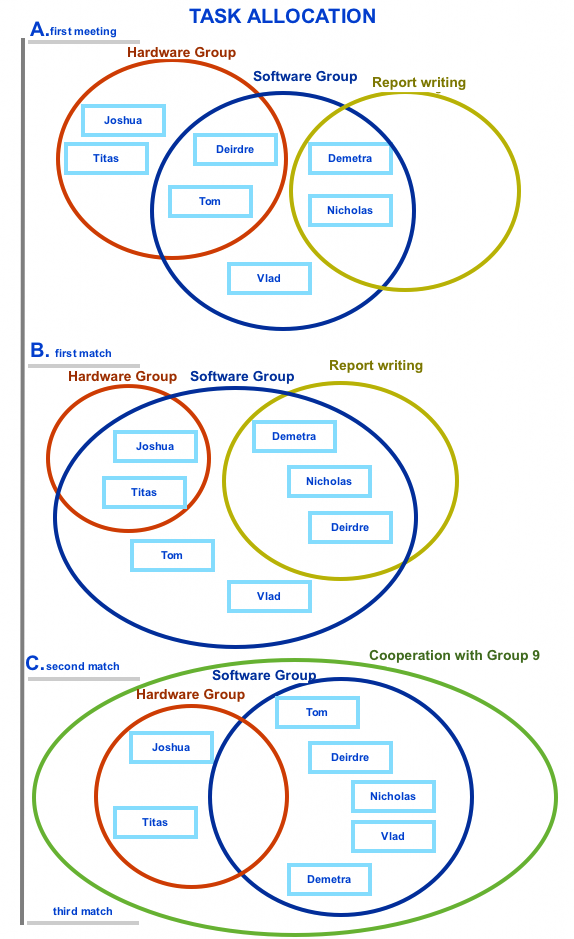
\includegraphics[width=16cm, height=17cm]{task_allocation.png}\\
		\caption{Diagram displaying how each member of the group is part of smaller group indicating the tasks to be done before each friendly match. Circles indicate the sub-groups that group 10 forms.}
	\end{minipage}%
\end{figure}


\subsection{Meetings}
Meetings are a vital component to the organisational structure of a group-based project, as this is where we can all discuss the progress we've made and the issues that have come up. Once a week, we meet with our mentor to relay how the group is progressing as a whole, as well as receive advice regarding the project. Additionally, sub-groups meet throughout the week to work on their assigned tasks. The progress made is noted in our Slack channel. Once we have collaborated with the group 9 in our group, we will also organise group meetings where both groups will come together and discuss ongoing changes and how to implement our tactics for match day.

\subsection{Tracking Progress}
Tracking progress is done through meetings as discussed above but also through our slack channel and Git repository. Each group member should have a task assigned to them which they should have completed by X date. Up to the set deadline each member will updated the group on their work and whether or not they are dealing with problems which may delay the deadline. When such issues arise a group member who may have completed, or is close to completing their task can help the other group member to solve the problem. When facing problems, we are all in the group together to help troubleshooting and keep our project on track.

\subsection{Git Repository}
Working as a group means many changes will be made on the code as each individual makes changes to code. To avoid code others have written being overwritten, a Git repository was created where the master branch is the original code, and from there when group members make changes to code they save it in a separate branch with a title corresponding to the changes made. This way everyone can keep track of what changes are being made. This also helps in tracking progress made towards our next milestone.


\section{Individual milestones and group tasks}
Each individual in the group will set themselves personal or group targets if they are working in a group of two for milestones set by them. For example if two people are working on the strategy of the robot, then the first milestone would be to have a basic strategy for the first Friendly game. As a group our first Milestone is having a working robot by Monday 30th January which will be able to perform in the first friendly. This will give us time to make adjustments to problems we encounter on the robot before the first friendly. 

As a group we have also set ourselves 'group Milestones' where we have a target day to have completed a certain functionality of the robot. This will give everyone the encouragement needed to push for their personal milestones so as when the group Milestone is reached all members of the group have their contribution towards this. 

We have decided to have practice games with the group 9 in our group as this will benefit both groups for testing the robots. It will also help us decide on what strategies we will implement when we have to work as a group on match day as through these practice games we will have a good understanding of each group's strengths and weaknesses. For example, if our group is better at defending than attacking or vice-versa then this will influence which robot will defend or attack on match day.

Individual and group milestones can be found in the figures 3 and 4 in the section "Gantt Charts", were are displayed using the symbol "*".

\section{Gantt Charts}
For better organisation of the group we decided to use Gantt charts. For this purpose we are using "Smartsheet" on-line tool. These charts will help us to complete the individual milestones faster and always be aware of what tasks are to be done and until when. Although we are aware that the plan is possibly going to change through the process, we created these charts to help us organising the work. As we are approaching the first and the second friendly match, we created two detailed Gantt charts, as we already know what needs to be done. For the weeks coming after these matches, we created more general Gantt charts because we cannot predict in detail what the workload will be. 


\subsection{Tasks until first friendly match}
In this detailed Gantt chart illustrated below, the tasks and milestones that need to be completed before the first friendly match are shown. In the first week, we had a general meeting on Wednesday where we met with our group members. We then separated into software and hardware groups and attended the corresponding workshops. After the workshops tasks for each individual in the group where assigned and each one started working on their allocated tasks.


The hardware group was responsible for building the basic robot structure, the kicker and catcher of the robot and then testing each part of the hardware. Meanwhile, the software group focused on the code from previous years so that they could modify it later. After the basic structure has finished, the software group cloned "Fred's" code and after testing it, proceeded to implementing the kicker and the catcher code. Through trial and error and many tests, the software and the hardware group adjusted the robot until the first friendly match that took place on 01/02/2017. Several issues came up such as a faulty Arduino and also several members of the Group becoming ill. This did not affect our deadlines time-line though as we planned for such issues in our risk assessment (see section 5).


\begin{figure}[H]
	\centering
	\begin{minipage}{1\textwidth}
		\centering
		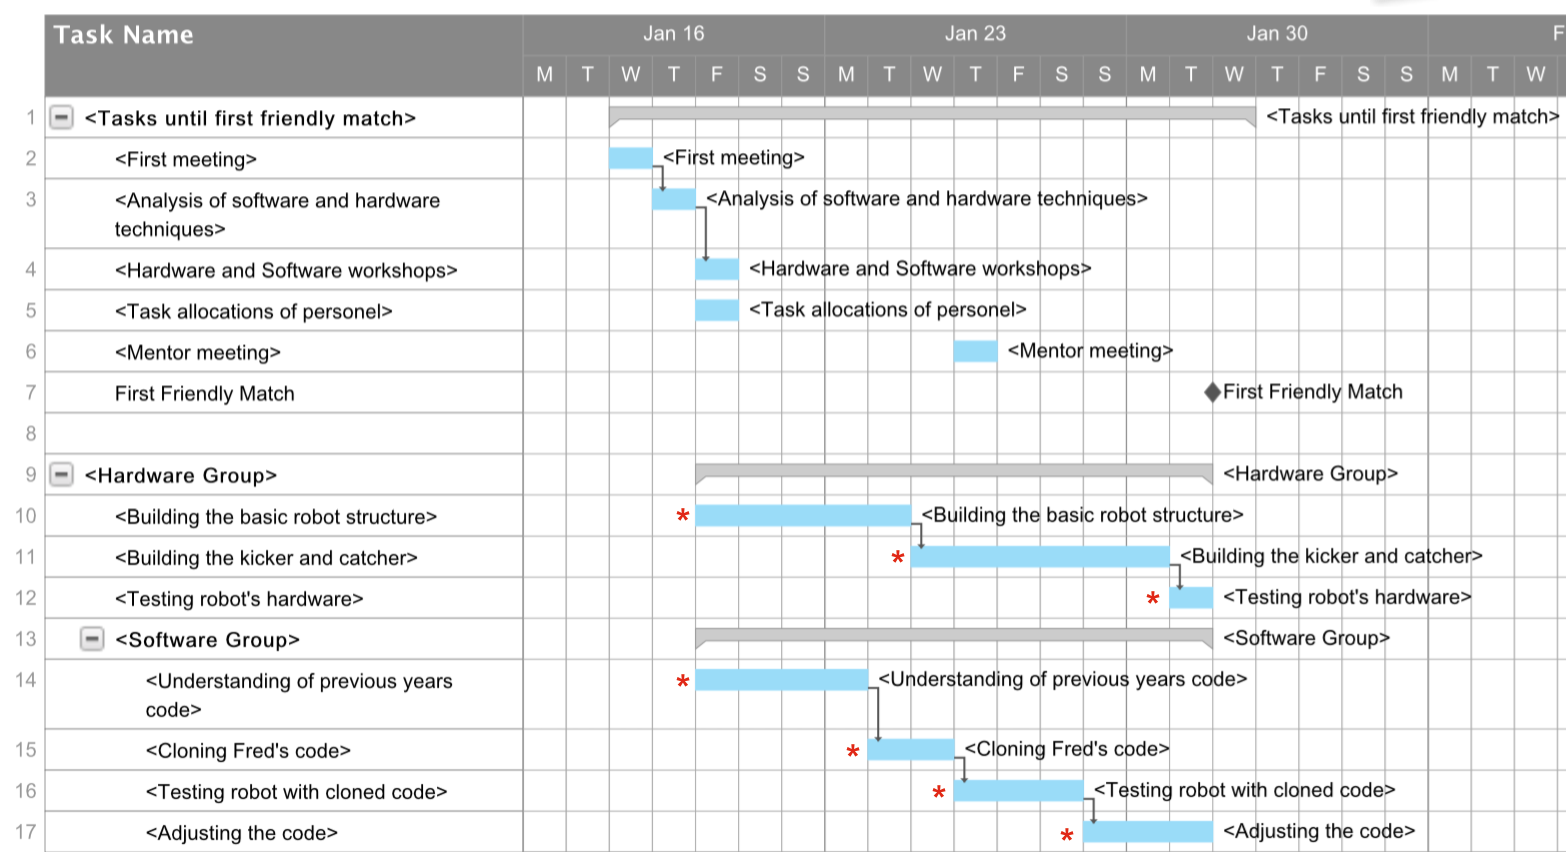
\includegraphics[width=16cm, height=10cm]{FirstFriendlyMatch.png}\\
		\caption{Gant chart illustrating the group tasks until the first friendly match (Milestones are indicated with symbol "*")}
	\end{minipage}%
\end{figure}

\subsection{First Match Review and tasks until second friendly match}
The results of the first match were three draws and one loss. The problematic areas were with the vision system and our kicker as we did not manage to score. The grabber worked well but needs improvement.
For our second friendly match, we aim to adjust the issues discussed above. Taking into account the performance of the robot in the first friendly match, we observed that we need to change our strategy and improve the implementation of the catcher and the kicker. The robot was able to move around the pitch, though it found self-recognition difficult due to the high reflection of the plates. As the vision system that we are using is considered a successful implementation we are not planning to change it until we observe its reaction with the new robot plates. As for the catcher and the kicker we decided that we are going to lower the catcher's motors power when shooting the ball and increase the kicker's power so that the ball can move on a straight line. We are also considering changing the batteries and adding more powerful ones as our robot needs a pack of batteries for both the wheels and the kicker. That will decrease the weight of the robot and it will move more smoothly on the pitch. In our second mentor meeting we discussed these improvements with our group mentor and we analyzed the procedure of writing the process report. We all agree that from this point, hardware group should start contributing with the software as there are not many hardware changes need to be made. After adjusting the software we are planning to test our robot in both pitches before the second friendly match. We are also planning an early-group meeting which will include members of group 9 that we are going to cooperate with on the third friendly match.

\begin{figure}[H]
	\centering
	\begin{minipage}{1\textwidth}
		\centering
		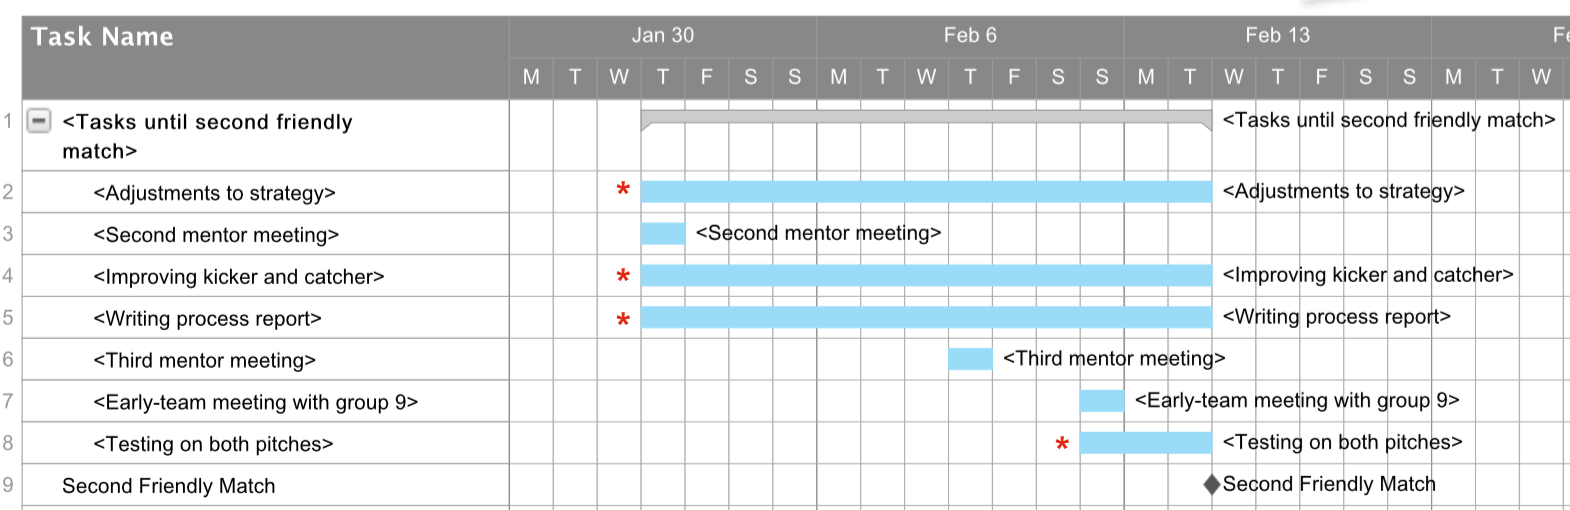
\includegraphics[width=16cm, height=7cm]{SecondFriendlyMatch.png}\\
		\caption{Gant chart illustrating the group tasks until the second friendly match (Milestones are indicated with symbol "*")}
	\end{minipage}%
\end{figure}


\subsection{Second Match Review and Tasks until third friendly match}
*Performance of robot in second match to be added
After completing the second friendly match we created a general approach for the tasks needing completion until the third friendly match. This match is where we are going to cooperate with group 9. Thus, we are planning to change our tactics before the third match and meet with the other group so that we can organise our strategy better. Meanwhile, we are going to have two of the weekly mentor meetings and our group meeting. While our groups are adjusting the code we are planning to have some practice matches with other groups to observe if the two robots are cooperating successfully in the field. Figure 5 illustrates these tasks with their corresponding dates.
\begin{figure}[H]
	\centering
	\begin{minipage}{1\textwidth}
		\centering
		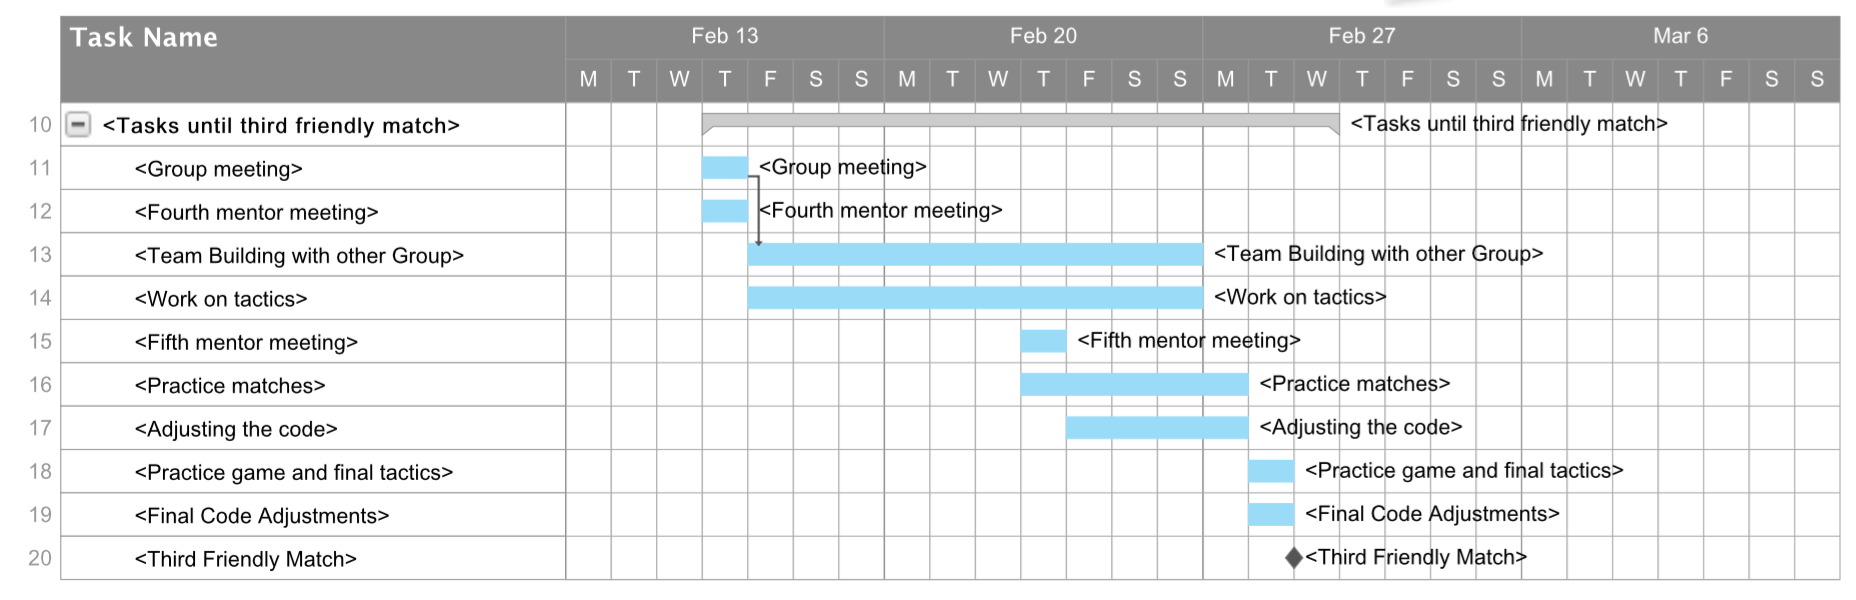
\includegraphics[width=16cm, height=7cm]{ThirdFriendlyMatch.png}\\
		\caption{Gant chart illustrating the group tasks until the third friendly match (Milestoned indicates with a *)}
	\end{minipage}%
\end{figure}

\subsection{Tasks until fourth friendly match}
Depending on the results of the third friendly match, we are going to have a group meeting discussing our robot's progress and a team meeting involving group 9 as well, to discuss our overall performance. Then, we will possibly have to adjust the code to improve any weaknesses of our robot and reform each group depending on the strategies chosen. Between the third and the fourth match we are basically going to work on the software and hardware to make our team cooperate in the best way. If we are satisfied with our performance, allocated members of the group will start writing the User Guide and the Technical report. In addition, we are going to have three more mentor meetings during this period. These tasks can be found in Figure 6.

\begin{figure}[H]
	\centering
	\begin{minipage}{1\textwidth}
		\centering
		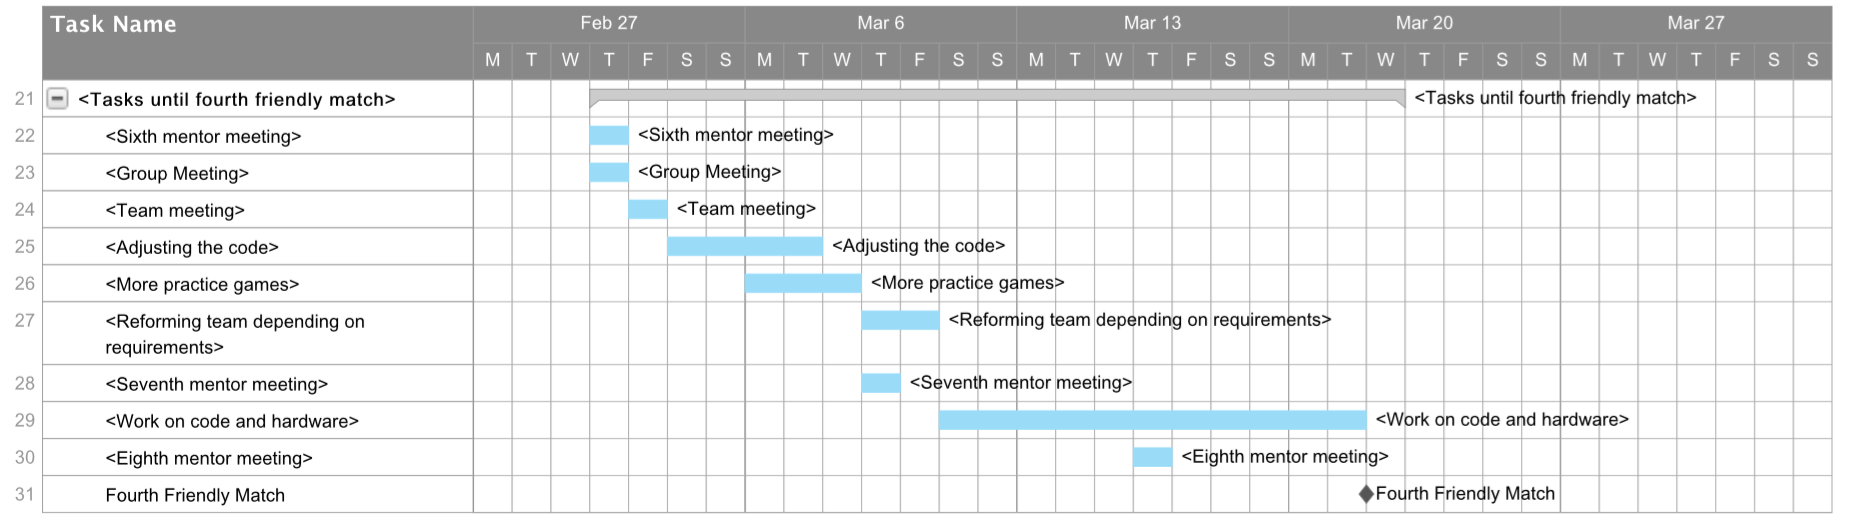
\includegraphics[width=16cm, height=7cm]{FourthFriendlyMatch.png}\\
		\caption{Gant chart illustrating the group tasks until the fourth friendly match}
	\end{minipage}%
\end{figure}

\subsection{Tasks until final day}
Before the final day, we will have to start preparing our presentations as well as the user guide and the technical report. Following the fourth friendly match, we are going to have the final adjustments in our code and discuss any possible changes on the strategy part with group 9. Until the final day we are going to have another three meetings with our mentor to guide us towards our presentation and any possible changes we can make. These tasks are presented in Figure 7.
\begin{figure}[H]
	\centering
	\begin{minipage}{1\textwidth}
		\centering
		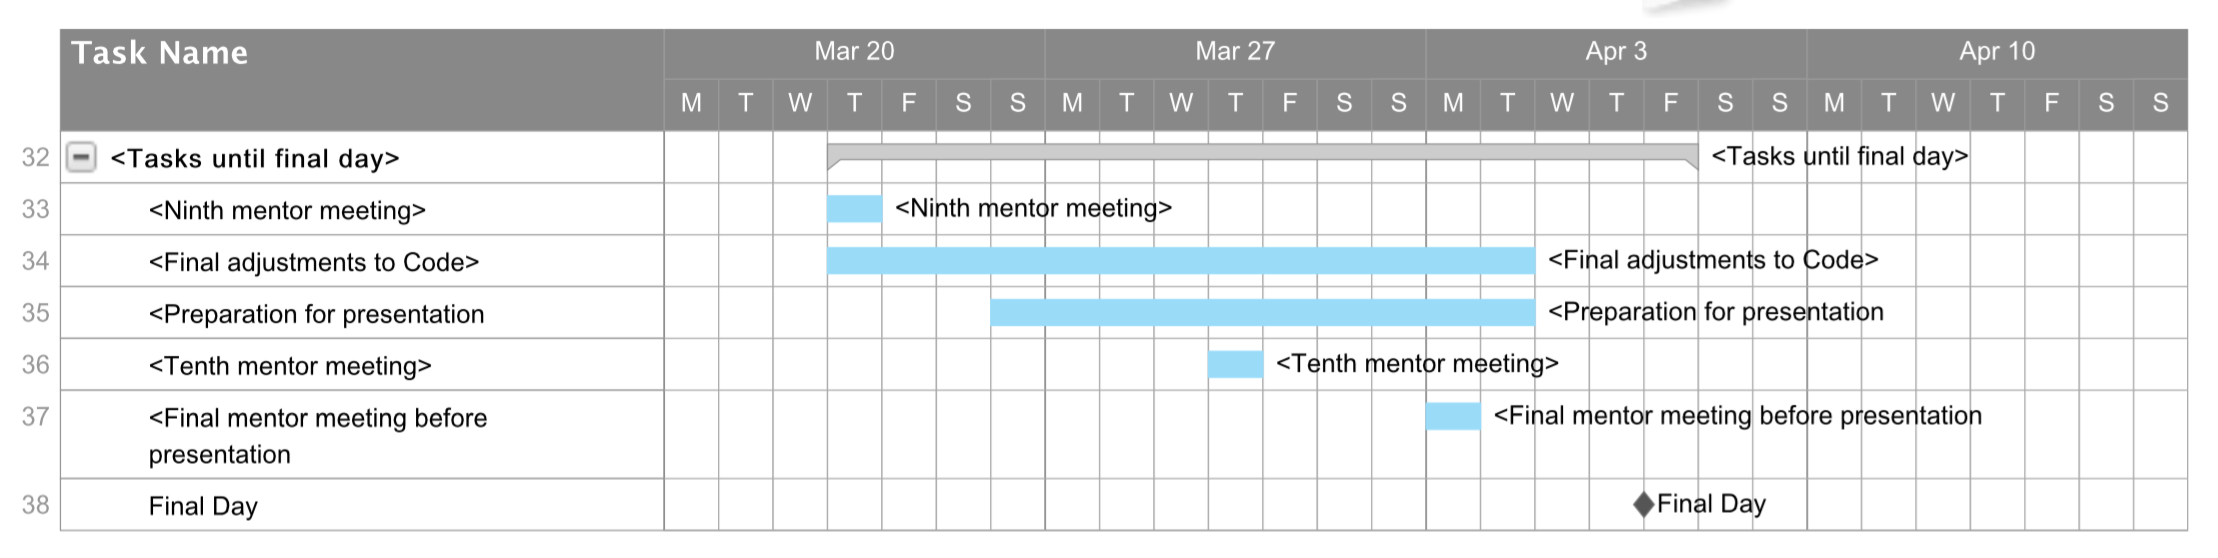
\includegraphics[width=16cm, height=7cm]{FinalDay.png}\\
		\caption{Gant chart illustrating the group tasks until final day}
	\end{minipage}%
\end{figure}

\section{Risk Assessment}
A risk assessment is crucial as it forms an integral part of a successful project. The main objectives are to identify what issues we may encounter along the way and how we will deal and adapt to these issues.
To try and discover as many risks we may be subject to over the course of the project, during a group meeting we sat down and brainstormed different risks we may face and thought of how we could deal with these. This helped in our planning of how to tackle the project.
Issues which we may come across which may backtrack our progress are shown in Figure 8.
\\include; a malfunction in the hardware such an Arduino breaking and needing replaced, needing to redesign the robot because of a very specific issue which the robot cannot be adapted to, a group member becoming ill and not being able to work pushing the work they were on back, a problem with the cameras in the pitch rooms which will backtrack testing and the pitch rooms being to busy for testing our robot again leading to delayed development.

With a well implemented risk assessment we can avoid these issues causing a delay in our planned timescale. To take into account of these risks we have taken several precautions. These precautions include; providing more time than is needed to completing tasks so that if any issues were to arise we would still be within the timescale as we have allocated time for these issues, if a group member were to become ill then there is another group member who is working closely with them on the same topic who can cover some of their work, and if there are any issues with overcrowding within a pitch room we focus on other tasks such as report writing or hardware fixes until the pitch rooms become available again. 

\section{Conclusion}
The project is currently proceeding on schedule in the second stage of it, up until the second friendly match. It is fully expected that the project will be completed on time.
The report contained an overview of how progress is being made on the project, what deliverables we have promised by certain dates and progress in relation to completed and upcoming tasks. The preceding analysis of the project has helped identify areas of improvement such as having more knowledge around robotics would help us design a robot in less time allowing for other improvements and also a reducing the time needed for a variety of tasks. Overall, all group members are putting great effort into this project and have all gained a great deal of knowledge from it.
 
\end{document}